\documentclass[a4paper, 12pt]{article}
\usepackage[osf]{libertinus} %font generale del documento
\pagestyle{plain} %nessxun heading o foot particolare
\usepackage[fontsize=13pt]{scrextend} %dimensione font 
\usepackage[a4paper,top=3cm,bottom=3cm,left=3cm,right=3cm]{geometry} %impaginazione e margini documento
\usepackage{graphicx, wrapfig} %gestione immagini e grafiche
\usepackage[ruled,vlined]{algorithm2e}
\usepackage{amsmath}
\usepackage{amsfonts}
\usepackage{float}

\newtheorem{theorem}{Teorema}
\newtheorem{definition}{Definizione}
\newtheorem{prop}{Proposizione}
\newtheorem{corollary}{Corollario}

\DeclareMathOperator\arccosh{arccosh}
\DeclareMathOperator\arcsinh{arcsinh}

\begin{document}

\begin{titlepage} %crea l'enviroment
\begin{figure}[t] %inserisce le figure
    \centering
\includegraphics[width=0.25\textwidth]{logo_unipg}
\end{figure}
\vspace{20mm}

\begin{Large}
 \begin{center}
	\textbf{Dipartimento di Matematica e Informatica\\ Corso di Laurea Triennale in Informatica\\}
	\vspace{20mm}
    {\LARGE{TESI DI LAUREA}}\\
	\vspace{10mm}
	{\huge{\bf Metodi di ottimizzazione su varietà differenziabili per la media di Fréchet su disco di Poincaré}}\\
\end{center}
\end{Large}

\vspace{30mm}
%minipage divide la pagina in due sezioni settabili
\begin{minipage}[t]{0.47\textwidth}
	{\large{\bf Relatore:\\ Bruno Iannazzo}}
\end{minipage}
\hfill
\begin{minipage}[t]{0.47\textwidth}\raggedleft
	{\large{\bf Candidato: \\ Luca Moroni\\ }}
	\vspace{5mm}
	{\large{\bf Matricola: \\ 311279\\ }}
\end{minipage}

\vspace{25mm}

\hrulefill

\vspace{5mm}

\centering{\large{\bf Anno Accademico 2020/2021 }}

\end{titlepage}

\clearpage
\begin{center}
    \thispagestyle{empty}
    \vspace*{\fill}
    Alla mia famiglia ed alla loro estrema pazienza.
    \vspace*{\fill}
\end{center}
\clearpage


\newpage

\renewcommand{\contentsname}{Contenuti}
\tableofcontents

\newpage

\section{Introduzione}
Le applicazioni pratiche nelle quali è necessario effettuare ottimizzazione di funzioni non lineari, ovvero trovarne un valore di minimo, nei giorni d'oggi sono molteplici. In particolare sono alla base del funzionamento di tecnologie molto utilizzate, tra cui le reti neurali, il cui apprendimento pone le fondamenta sulla solida teoria matematica dei metodi numerici per l'ottimizzazione.\\
Negli ultimi anni si sta affermando una generalizzazione dell'ottimizzazione classica dove la funzione da ottimizzare non ha come dominio un sottoinsieme dello spazio euclideo ma una varietà differenziabile. le applicazioni di queste nuove tecniche sono moltissime: possiamo pensare ad esempio al calcolo di autospazi di una matrice, che rappresenta un problema molto comune e necessario da risolvere in molte applicazioni dell'algebra lineare; possiamo pensare al problema della decomposizione SVD il quale può essere modellizzato come un problema di ottimizzazione su varietà. un altro problema è l'analisi delle componenti indipendenti, Indipendent Component Analysis (ICA), conosciuto come separazione delle sorgenti e modellizzabile anch'esso come un problema di ottimizzazione su varietà, il quale ha ricevuto un forte interesse nella ricerca di questi ultimi anni dato dall'ampia applicazione nell'ambito biomedico.\\
L'applicazione su cui si basa la tesi è il calcolo del centroide di $p$-punti in una varietà riemanniana, che può essere posto come un problema di ottimizzazione sulla varietà stessa, infatti è il minimo della funzione somma delle distanza al quadrato dai punti dati, questo problema ammette un unico minimo, questo accade in particolare per il disco di Poincaré che è una famosa varietà riemanniana, che è forse il più famoso modello di geometria non euclide con curvatura negatiava, verrà confrontata la risoluzione di tale problema con il corrispettivo problema trasferito nella varietà conforme iperboloide. Confonteremo vari algoritmi di ottimizzazione su varietà per calcolare il centroinde di p-punti, per questo faremo uso di metodi di discesa del gradiente, è importante notare che tali metodi non possono essere implementati in modo "naturale" come avviene nel caso euclideo, ma è necessaria una "codifica" del problema ed inoltre sono necessari particolari strumenti, che verranno trattati ed esplicitati nella presente, questo poichè, contrariamente al caso euclideo, il gradiente non appartiene allo stesso spazio su cui è definita la funzione da minimizzare ma in uno spazio tangente alla varietà che è uno spazio ben diverso, perciò la normale somma del gradiente non garantirebbe il corretto funzionamento dei metodi che descriveremo, tra i quali sono presenti l'algoritmo a passo fisso, ricerca lineare ed altri più performanti.\\
Tale sperimentazione prende spunto dall'articolo \cite{Wilson}, il nostro contributo consiste nel considerare una più ampia gamma di algoritmi tra cui il metodo di Barzilai Borwain riemanniano recentemente introdotto in \cite{Iannazzo} dove viene mostrata la sua efficienza nel calcolo del centroide nella varietà delle matrici definite positive. I nostri esperimenti mostrano che anche nel caso del disco di Poincaré e dell'iperboloide questo algoritmo è estremamente più efficiente dei metodi classici del gradiente con ricerca lineare o passo fisso.\\
Capiremo inoltre se tali modelli conformi sono equivalenti, non solo da un punto di vista geometrico ma anche sotto un aspetto computazionale tale per cui effettuare ottimizzazione. Inoltre tale trattazione vuole far comprendere la possibilità, in problemi di ottimizzazione su varietà, di interscambiare modelli conformi. Gli esperimenti trattati vorrebbero, infine, dare l'incipit per continuare con altre sperimentazioni analoghe andando, magari, a trattare anche il modello del semipiano di Poincaré.

\section{Metodi di ottimizzazione su $\mathbb{R}^n$ e varietà differenziabili}
Nella presente trattazione i vettori verranno indicati tramite le ultime lettere minuscole dell'alfabeto $x, v, w$, che assumeremo essere vettori colonna, il trasposto di un vettore verrà identificato tramite il carattere apice ($'$) perciò per definire il prodotto scalare euclideo di due vettori $u, v$ scriveremo $u'v$, mentre se si intende  un prodotto scalare differente da quello euclideo, come è il prodotto scalare riemanniano, lo indicheremo con $\langle \cdot,\cdot \rangle$, ricordiamo che il prodotto scalare in una varietà riemanniana dipende da un punto nella varità.\\
In tale sezione andremo ad esplicitare le metodologie generali per trovare un minimo di una funzione $f$ definita su una varieta differenziabile $M$ a valori reali (notiamo che $\mathbb{R}^n$ è un caso particolare di varietà differenziabile). Cercheremo di trovare quei punti che garantiscono l'ottimalità di una funzione, ovvero punti di massimo e di minimo, che descriveremo a breve.\\
Sia $f: \mathbb{R} ^n \to \mathbb{R}$ non vincolata.
Un vettore $x^\ast$ è un minimo locale non vincolato per la funzione $f$ se, informalmente, $f$ assume un valore in $x^\ast$ non più grande dei valori che assume in un intorno di $x^\ast$ stesso. Più formalmente $x^\ast$ è minimo locale per $f$ se esiste $\epsilon > 0$ tale che,\\
\[f(x^\ast) \leq f, \mbox{ per ogni } x \mbox{ con } \parallel x - x^\ast \parallel < \varepsilon,\]\\
$\| x \|$ rappresenta la norma euclidea del vettore $x$.\\
Un vettore $x^\ast$ è un minimo globale non vincolato rispetto ad $f$ se la funzione assume un valore in $x^\ast$ non più grande dei valori che assume in ogni altro vettore nel proprio dominio, più formalmente $x^\ast$ è tale che\\
\[f(x^\ast) \leq f, \mbox{ per ogni } x \in \mathbb{R}^n.\]\\
\subsection{Condizioni necessarie per l'ottimalità}
Se la funzione di costo $f$ è differenziabile, possiamo utilizzare il gradiente e l'espansione in serie di Taylor per comparare il costo di un vettore con il costo di un suo intorno.
Ci aspettiamo perciò che se $x^\ast$ è un minimo non vincolato allora la variazione della funzione al primo ordine per una piccola variazione $\Delta x$ è non negativa\\
\[\nabla f ( x^\ast )' \Delta x \geq 0.\]\\
Perciò valendo sia per $\Delta x$ positivi che negativi abbiamo la seguente condizione necessaria,\\
\[\nabla f ( x^\ast )' = 0. \]\\
Ci aspettiamo inoltre che anche la variazione della funzione al secondo ordine per una piccola variazione di $\Delta x$ è non negativa,\\
\[\nabla f ( x^\ast )' \Delta x + (1/2) \Delta x' \nabla ^2 f (x^\ast) \Delta x\geq 0,\]\\
dato che la precedente osservazione ha imposto $\nabla f (x^\ast)' \Delta x = 0$ otteniamo che\\
\[\Delta x' \nabla ^2 f (x^\ast) \Delta x\geq 0,\]\\
e che perciò\\
\[\nabla ^2 f (x^\ast) \mbox{ è una matrice semidefinita positiva.}\]\\
Diamo il seguente risultato che sintetizza quanto detto fin'ora.
\begin{prop}[Condizioni necessarie di ottimalità]
Sia $x^\ast$ un minimo locale non vincolato di $f:\mathbb{R}^n \to R$, assumiamo $f$ differenziabile con continuità in un insieme aperto $S$ contenente $x^\ast$. Allora\\
\[\nabla f(x^\ast) = 0,\]\\
Se $f$ è due volte differenziabile con continuità in $S$, allora\\
\[\nabla^2 f(x^\ast) \mbox{ è una matrice semidefinita positiva.}\]
\end{prop}
\subsection{Il caso della convessità}
Se la funzione $f$ è convessa su un insieme convesso non ci sono distinzioni tra un minimo locale ed un minimo globale, tutti i punti di minimo locale sono anche punti di minimo globale. Perciò un fatto importante è che la condizione $\nabla f(x^\ast) = 0$ è sufficiente per l'ottimalità, da cui deriva il seguente risultato.
\begin{prop}[Funzioni Convesse] Sia $f:\mathbb{R}^n \to R$ una funzione convessa su un insieme convesso $X$.
\begin{itemize}
  \item Un minimo locale di $f$ su $X$ è anche un minimo globale su $X$. Se inoltre $f$ è strettamente convessa, allora esiste al più un minimo per $f$.
  \item Se $f$ è convessa e l'insieme $X$ è aperto, allora $\nabla f(x^\ast) = 0$ è una condizione necessaria e sufficiente per il vettore $x^\ast \in X$ per essere minimo globale di $f$ su $X$.
\end{itemize}
\end{prop}

\subsection{Condizioni Sufficienti per l'ottimalità}
Non è difficile trovare esempi in cui le condizione di ottimalita necessarie definite nelle sezione precedente
[$\nabla f(x^\ast) = 0 \quad \mbox{e} \quad \nabla^2 f(x^\ast) \geq 0$]
portino ad identificare punti che non sono di minimo locale come ad esempio punti di sella o punti di massimo.\\
Supponiamo di avere un vettore $x^\ast$ che soddisfa le seguenti condizioni\\\\
- $\nabla f(x^\ast) = 0$.\\
- $\nabla^2 f(x^\ast)$ è una matrice definita positiva.\\\\
Allora abbiamo che per ogni $\Delta x \neq 0$ con $\Delta x \in \mathbb{R}^n \setminus \{0\}$\\
\[\Delta x' \nabla^2f(x^\ast) \Delta x > 0.\]\\
Ciò implica che in $x^\ast$ la variazione di $f$ al secondo ordine data da un piccolo spostamento $\Delta x$ è positiva, perciò $f$ tende ad incrementare nell'intorno di $x^\ast$ e ciò implica che le due condizioni di cui sopra sono necessarie e sufficienti per l'ottimalità locale di $x^\ast$.
\begin{prop}[Condizioni di ottimalità sufficienti del secondo ordine] Sia $f:S \subset \mathbb{R}^n \to R$ derivabile due volte con continuità. Si supponga che esista $x^\ast \in S$ che soddisfi le condizioni\\
\[\nabla f(x^\ast) = 0 \quad \mbox{e} \quad \nabla^2 f(x^\ast) \mbox{è una matrice definita positiva.}\]\\
Allora, $x^\ast$ è un minimo locale di $f$. In particolare esistono $\gamma > 0$ e $\epsilon > 0$ tali che\\
\[ f(x) \geq f(x^\ast) + \frac{\gamma}{2} \parallel x - x^\ast \parallel^2, \quad \mbox{per ogni} x \quad \mbox{con} \parallel x - x^\ast \parallel < \epsilon  \]
\end{prop}
\subsection{Discesa del gradiente in $\mathbb{R}^n$}
Andiamo ora a definire nel dettaglio le principali metodologie computazionali di ottimizzazione non lineare su $\mathbb{R}^n$. Tali metodologie sarannno trattate con un occhio alle possibili applicazioni.\\
Consideriamo il problema di trovare il minimo non vincolato di una funzione $f:\mathbb{R}^n \to R$. Nella maggior parte di casi non è possibile trovare una soluzione analitica, perciò l'approccio adottato è quello di applicare un algoritmo iterativo chiamato \textit{iterative descent} che opera come segue: prendiamo un vettore iniziale $x^0$ e successivamente generiamo una sequenza $x^1, x^2, ...$ tale che $f$ decresce ad ogni iterazione $f(x^{k+1}) < f(x^k)$ e sperabilmente converga un punto di minimo.\\
I principali algoritmi di discesa sono metodi del gradiente poichè sono basati sul gradiente della funzione $f$.
\subsubsection{Selezionare la direzione di discesa}
Sia $v \in \mathbb{R}^n \setminus 0$, $v^\perp$ è un iperpiano, contenente i punti tali che $v'd = 0$, divide lo spazio in due componenti connesse:
\begin{itemize}
  \item $v'd > 0$ (semipiano).
  \item $v'd < 0$ (semipiano).
\end{itemize}
Se $v = \nabla f(x)$ ogni $d$ tale che $v'd < 0$ è una direzione di decrescita, come mostrato nel seguente teorema.
\begin{theorem}
Sia $f \in C^1(\Omega)$, con $\Omega$ aperto di $\mathbb{R}^n$ e sia $x \in \Omega$ e $\nabla f(x) \neq 0$ per ogni $d \in \mathbb{R}^n$ tale che $\nabla f(x)'d < 0$ ed esiste $\alpha^0 > 0$ tale che $f(x + \alpha d) < f(x)$ con $\alpha \in (0, \alpha^0]$
\end{theorem}
Detto ciò possiamo dare una classe di algoritmi con $x^0 \in \Omega$ e dove $d_k \in \mathbb{R}^n$ è detta direizione ed $\alpha_k$ è detto passo, definiti secondo la seguente formula,\\
\[x^{k+1} = x^k + \alpha^k d^k \quad k=0, 1, ... ,\]\\
Dove se $\nabla f(x^k) \neq 0$ la direzione $d^k$ è scelta in modo tale che\\
\[\nabla f(x^k)'d^k < 0.\]\\
Ci sono varie possibilita nella scelta di $d^k$ e di $\alpha^k$.\\
Molti metodi di gradiente sono definiti nella forma,
\[x^{k+1} = x^k - \alpha^k D^k \nabla f(x^k),\]
dove $D^k$ è una matrice definita positiva e con $d^k = -D^k\nabla f(x^k)$ allora è immediato verificare che $\nabla f(x^k)'d^k < 0$.\\
A seconda della scelta di $D^k$ abbiamo differenti metodi applicabili.\\\\
\begin{itemize}
    \item \textbf{Steepest Descent}: $D^k = I, \quad k = 0, 1, ...$.
    \item \textbf{Metodi di Newton}: $D^k = (\nabla^2 f(x^k))^{-1}, \quad k = 0, 1, ...$, $\nabla^2 f(x^k)$ deve essere definita positiva, proprietà sempre verificata se $f$ è convessa.
    \item \textbf{Steepest Descent Riscalata}: $D^k$ matrice diagonale.
    \item \textbf{Metodi di Schamansky}: $D^k = (\nabla^2 f(x^0))^{-1}$.
    \item \textbf{Metodi di quasi Newton}: $D^k = H(x^k) \approx \nabla^2 f(x^k)$.
\end{itemize}
Nonostante i metodi di Newton convergono molto velocemente, non sono utilizzati nella pratica dal momento in cui il calcolo della matrice hessiana è computazionalmente oneroso, perciò sono stati introdotti i metodi di quasi Newton, nel qual caso la matrice $D^k$ è scelta in modo tale che la direzione $d^k = -D^k\nabla f(z^k)$ tenda ad approssimare la direzione del metodo di Newton, e $D_k$ approssima la matrice hessiana. L'idea fondamentale riguardo questa metodologia è che tramite due iterate successive $k$, $k+1$ ed i valori $x^k$, $x^{k+1}$, $\nabla f(x^k)$, $\nabla f(x^{k+1})$ noi possiamo avere accesso a delle informazioni riguardo la matrice hessiana, in particolare abbiamo che\\
\[\nabla f(x^{k+1}) - \nabla f(x^k) \approx H(x^{k+1})(x^{k+1} - x^k).\]\\
Definiti $p^k = x^{k+1} - x^k$ e $q^k = \nabla f(x^{k+1}) - \nabla f(x^k)$ allora $D^{k+1}$ deve soddisfare l'uguaglianza $D^{k+1} p^k = q^k$, questo prende il nome di equazione delle secanti.
\subsubsection{Selezione del passo}
Ci sono numerose metodologie per la scelta del passo $a^k$ nei metodi del gradiente, ne elenchiamo alcune.\\\\
\textbf{Ricerca lineare esatta}:\\
scegliamo $\alpha^k$ tale che minimizza la funzione costo $f$ lungo la direzione $d^k$, perciò,\\
\[f(x^k + \alpha^k d^k) = \min_{\alpha \geq 0} f(x^k + \alpha d^k).\]\\
\textbf{Ricerca lineare esatta limitata}:\\
Questa è una versione modifica della metodologia precedente più semplice da implementare in vari casi. definito un scalare $s > 0$ $\alpha^k$ è scelto in modo tale che minimizza il costo di $f$ nell'intervallo $[0, s]$,\\
\[f(x^k + \alpha^k d^k) = \min_{\alpha \in [0, s]} f(x^k + \alpha d^k).\]\\
Le due metodologie appena presentate sono solitamente implementate con l'aiuto delle tecniche risolutive dell'ottimizzazione in una variabile, che è un problema certamente più facile da risolvere in modo analitico.\\\\
\textbf{Metodo di Armijo}:\\
Scegliere $\alpha^k$ in modo che garantisca una decrescita sufficiente a garantire la convergenza del metodo sotto opportune ipotesi. Il metodo di armijo è stato definito come segue. Siano fissati $\lambda, \sigma$ e $\gamma$ con $0 < \sigma < 1$, e $0 < \gamma < 1$ e sia $\alpha^k = \sigma^{m_k} \lambda$, dove $m_k$ è il primo intero non negativo per cui vale\\
\[f(x^k) - f(x^k + \sigma^m \lambda d^k) \geq -\gamma \sigma^m \lambda \nabla f(^k)'d^k.\]\\
Solitamente si scelgono i valori come segue, $\gamma \in [10^{-5}, 10^{-1}]$, il fattore di riduzione $\sigma \in [1/10, 1/2]$, possiamo scegliere $s = 1$ e moltiplicare la direzione $d^k$ per uno scalare.\\
Per questa metodologia diamo anche il seguente teorema che rappresenta un risultato importante.
\begin{definition}
Una successione di direzioni $\{d^k\}_k$ è detta limitata se vale la seguente,\\ \[\parallel d^k \parallel < M \mbox{ per ogni } k \mbox{ con } M \in \mathbb{R}^+.\]
\end{definition}
\begin{definition}
Una successione di direzioni $\{x^k\}_k, \quad \{d^k\}_k$ è detta \textbf{gradient related} se per ogni sotto-successione di $\{x^k\}_k$ che converge ad un punto non stazionario $\{d^k\}_k$ è limitata ed inoltre vale,\\
\[\limsup\limits_{k \in K} \nabla f(x)'d^k < 0.\]
\end{definition}
Ora diamo il principale risultato che garantisce la convergenza globale per metodi di discesa che utilizzano la tecnica di Armijo.
\begin{theorem}
Sia $\{x^k\}_k$ una sequenza infinita (non definitivamente uguale al suo limite) generata dal metodo $x^{k+1} = x^k + \alpha^k d^k$, dove $\alpha^k$ è generato con la regola di armijo e $d^k$ è \textbf{gradient related}. Allora ogni punto limite è stazionario.
\end{theorem}
\textbf{Metodo a passo costante}:\\
Si definisce un passo costante $s > 0$ e si fissa $\alpha^k = s, \quad k = 0,1, ...$\\
Il passo costante è una metodologia veramente semplice da implementare ma si deve fare attenzione nella scelta del passo, se si sceglie un valore di $s$ troppo grande allora il metodo divergerà, contrariamente se il passo $s$ venisse scelto troppo piccolo l'ordine di convergenza risulterebbe troppo lento.\\\\
\textbf{Metodo di diminuzione del passo}:\\
Scegliamo il passo in modo tale che $\alpha^k \rightarrow 0$. Una problematica legata a questa metodologia è che il passo può diventare troppo piccolo per cui non può essere garantita la convergenza, per questa ragione viene richiesto che.\\ \[\sum_{n=1}^{\infty} \alpha^k = \infty.\]
\subsection{Discesa del gradiente su varietà} \label{riemanniangd}
Ora che abbiamo un contesto teorico e una consapevolezza di cosa voglia dire effetutare ottimizzazione su uno spazio euclideo $n$-dimensionale ($\mathbb{R}^n$), possiamo approcciare le metodologie computazionali per trovare un minimo non vincolato di una funzione $f:M \to R$ analoghe a quella definite nella sezione precedente. Prima di andare nel vivo del discorso dobbiamo però munirci degli strumenti necessari, richiamiamo la parte dedicata alle varietà differenziabili presente nell'appendice e aggiungiamo quanto segue.
\subsubsection{Retrazioni} \label{retraction}
Su varietà differenziabili la nozione di muoversi nella direzione del vettore tangente rimanendo nella varietà stessa è generalizzato dal concetto di \textbf{Retrazione}, concettualmente una retrazione $R$ su $x$, denominata come $R_x$, è una mappa che va da $T_xM$ (spazio tangente in $x$ rispetto a $M$) in $M$ con una condizione di rigidità locale che preserva il gradiente in $x$.
\begin{definition}[Retrazione]
Una retrazione in una varietà $M$ è una mappa liscia $R$ che ha come dominio l'insieme dei $T_xM \quad \forall x \in M$ in $M$ con le seguenti proprietà. Sia $R_x$ la restrizione di $R$ a $T_xM$.
\begin{itemize}
  \item $R_x(0_x) = x$, dove $0_x$ denota l'elemento zero (origine) di $T_xM$.
  \item Con l'identificazione canonica $T_{0_x} T_xM \simeq T_xM$, $R_x$ soddisfa\\
  $DR_x(0_x) = id_{T_xM},$\\
  dove $id_{T_xM}$ denota la mappa identità su $T_xM$.
\end{itemize}
\end{definition}
Ci riferiamo alla condizione $DR_x(0_x) = id_{T_xM}$ come condizione di \emph{rigidità locale}. Equivalentemente, per ogni vettore tangente $\xi$ in $T_xM$, la curva $\gamma_{\xi}:t \mapsto R_x(t\xi)$ soddisfa $\gamma_{\xi}(0)' = \xi$.\\
Oltre a trasformare elementi di $T_xM$ in elementi di $M$, un secondo importate scopo della retrazione $R_x$ è quello di trasformare una funzione costo ($f:M \to R$) definita in un intorno di $x \in M$ in una funzione costo definita sullo spazio vettoriale $T_xM$. Nello specifico, data una funzione reale $f$ su una varietà $M$ su cui è definita una retrazione $R$, abbiamo che $\hat{f} = f \circ R$ denota il $\emph{pullback}$ di $f$ attraverso $R$. Per $x \in M$, abbiamo che\\
\[\hat{f_x} = f \circ R_x\]\\
denota la restrizione di $\hat{f}$ su $T_xM$. Si noti che $\hat{f_x}$ è una funzione reale su uno spazio vettoriale. Dalla condizione di rigidità locale abbiamo che $D\hat{f_x}(0_x) = Df(x)$. Se $M$ è dotato di una metrica Riemanniana abbiamo\\
\[ \mbox{grad} \hat{f_x}(0_x) = \mbox{grad} f(x).\]\\
Un caso particolare di retrazione è la \textbf{mappa esponenziale} definita su $p \in M$ e $v \in T_pM$, che ha proprietà di retrazione, rappresenta la curva geodedica calcolata nel punto $1$ originaria in $p$ con derivata in $0$ punto pari a $v$.\\
In alcuni casi può essere necessario dover effettuare operazioni tra vettori appartenenti a spazi tangente diffenti, come ad esempio nel caso dei metodi di ottimizzazzione quasi Newton. Nell'ottimizzazione basata su retrazioni lo strumento standard per trasportare vettori appartenenti ad uno spazio tangente in un altro spazio tangente è il $trasporto vettoriale$. Informalmente, dati due vettori tangenti ad $x$, chiamati $v_x, w_x \in T_xM$, un trasporto vettoriale $\mathcal{T}$ associato ad una retrazione $R$, è una mappa liscia che genera un vettore appartenente ad $T_{R_x(w_x)}M$. Per semplicità utilizzeremo la notazione $\mathcal{T}_{x \to y}(v)$.\\
Un caso speciale di trasporto vettoriale è il $trasporto$ $parallelo$ che puo essere interpretato come un trasporto vettoriale la cui retrazione associata è la mappa esponenziale.
\subsubsection{Metodi \emph{line-search}} \label{riemannian_linesearch}
I metodi di ricerca in linea (definiti \emph{line-search}) su varietà si basano sulla formula di aggiornamento\\
$x^{k+1} = R_{x^k}(t^k \eta^k)$,\\
dove $\eta^k$ è in $T_xM$ e $t^k$ è uno scalare. Una volta scelta la retrazione $R$ ci rimane da decidere la direzione $\eta^k$ e la lunghezza del passo $t^k$. Per ottenere la convergenza del metodo delle restrizioni sulla scelta di questi due parametri devono essere fatte.\\
\begin{definition}[sequenza gradient related su varietà]
Data una funzione di costo $f$ su una varietà riemanniana $M$, una sequenza $\{\eta^k \}$, $\eta^k \in T_xM$ è \textbf{gradient related} se per ogni sotto-sequenza $\{x^k\}_{k \in K}$ di $\{x^k\}$ che converge ad un punto non stazionario di $f$, la corrispondente sotto-sequenza $\{\eta^k\}_{k \in K}$ è limitata e soddisfa\\
$\limsup\limits_{k \to \infty, k \in K} \langle$grad $f(x^k), \eta^k \rangle < 0$
\end{definition}
\begin{definition}[Punto di Armijo su varietà]
Data una funzione $f$ su una varietà riemanniana $M$ dotata di una retrazione $R$, un punto $x \in M$, un vettore tangente $\eta \in T_xM$, e degli scalari $\bar{\alpha} > 0, \beta, \sigma \in (0, 1)$, un \textbf{punto di Armijo su varietà} è $\eta^A = t^{A}\eta = \beta^{m}\bar{\alpha}\eta$, dove $m$ è il più piccolo intero non negativo tale che\\
$f(x) - f(R_x(\beta^{m}\bar{\alpha}\eta)) \geq -\sigma \langle$grad $f(x), \beta^m\bar{\alpha}\eta \rangle_x$.\\
Il valore reale $t^A$ è il \textbf{Passo di Armijo}.
\end{definition}
Andiamo ora a definire un algoritmo generico per la discesa di gradiente su varietà (\textbf{Accelerated Line Search}), tale algoritmo rappresenta una generalità di metodologie di ottimizzazione delineando però, nel contempo, delle restrizioni fondamentali che garantiscono la convergenza della sequenza di punti generati.\\
\begin{center}
\begin{algorithm}[H]
\SetAlgoLined
\KwIn{Manifold $M$; funzione costo $f$ differenziabile definita su $M$; retraction $R$; scalari $\bar{\alpha} > 0$, $c, \beta, \sigma \in (0,1)$; initial iterate $x^0 \in M$}
\KwOut{Sequenza $\{x^k\}$}
\For{$k=0, 1, 2, ...$}{
    Prendere $\eta^k \in T_xM$ tale per cui la sequenza $\{\eta^i\}_{i=0,1,...}$ sia \emph{gradient related}.\\
    Selezionare $x^{k+1}$ tale che
    \begin{equation}
    \label{ctr-als}
    \hspace{10mm}f(x^k)-f(x^{k+1}) \geq c(f(x^k)-f(R_{x^k}(t^{k^A}\eta^k)))
    \end{equation}
    Dove $t^{k^A}$ è il passo definito dalla regola di Armijo su varietà definita poco sopra.
}
\caption{Accelerated Line Search (ALS)}
\end{algorithm}
\end{center}
Dallo pseudocodice appena esplicitato è chiaro che tale algoritmo puo essere visto come una generalizzazione della scelta del passo di Armijo descritto nella sotto-sezione 2.2, difatti scegliere $x^{k+1} = R_{x^k}(t^{k^A}\eta^k)$ soddisfa \eqref{ctr-als}. Inoltre la condizione rilassata \eqref{ctr-als} ci permette un ampio spazio di manovra nella scelta di $x^{k+1}$ grantendoci la convergenza ad un punto stazionario, come enunceremo formalmente, e ciò puo portare alla definizione di algoritmi altamente efficienti.

\subsubsection{Convergenza}
Il concetto di convergenza puo essere ridefinito e generalizzato su varietà. Una sequenza infinita $\{x^k\}_{k=0,1,...}$ di punti su una varietà $M$ è detta essere convergente se esiste una carta $(U, \psi)$ di $M$, un punto $x^\ast \in M$ e $K > 0$ tali che $x^k$ è in $U$ per ogni $k \geq K$ e tale che la sequenza $\{\psi(x^k)\}_{x=K, K+1, ...}$ converge a $\psi(x^\ast)$ (in tal caso applichiamo il concetto di convergenza di $\mathbb{R}^n$, avendo $\psi$ come codominio uno spazio euclideo). Il punto $\psi^{-1}(\lim_{k \to \infty} \psi(x^k))$ è chiamato il \emph{limite} della sequenza $\{x^k\}_{k=0,1,...}$. Tutte le sequenze convergenti di una varietà di \emph{Hausdorff} hanno uno ed un solo punto limite.\\
Diamo ora un importante risultato rispetto alla convergenza dell'algoritmo \emph{ALS}, tale enunciato deriva direttamente dal risultato di convergenza definito nella sezione 2.2 rispetto al passo di Armijo in $\mathbb{R}^n$, in tal caso però viene data una generalizzazione di quest'ultimo essendo, come già detto, ALS una generalizzazione del passo di Armijo e lavorando non più su $\mathbb{R}^n$ ma su varietà differenziabili.
\begin{theorem}
Sia $\{x^k\}$ una sequenza infinita di iterate generate da ALS. Allora ogni punto di accumulazione  di $\{x^k\}$ è un punto stazionario della funzione costo $f$
\end{theorem}
Inoltre assumendo compattezza della varietà $M$ possiamo enunciare il seguente
\begin{corollary}
Sia $\{x^k\}$ una sequenza finita di iterate generata da ALS. Assumiamo che l'insieme di livello $L = \{x \in M : f(x) \leq f(x^0)\}$ è compatto allora\\ $\lim_{k \to \infty} \parallel $grad $f(x^k) \parallel = 0$.
\end{corollary}

\section{Disco di Poincaré e Iperboloide}
Lo spazio iperbolico può essere definito in vari modi equivalenti, noi descriveremo l'iperboloide ed il disco di Poincaré, ciascuno di questi è un modello dello spazio iperbolico, nessuno dei due è prevalente in letteratura.\\
\begin{figure}[t] %inserisce le figure
    \centering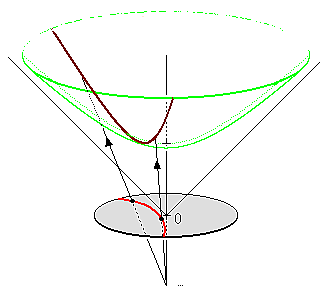
\includegraphics[width=0.50\textwidth]{HyperboloidProjection.png}
    \caption{Rappresentazione della proiezione stereografica tra disco e iperboloide}
\end{figure}
\subsection{Iperboloide}
Possiamo definire $\mathbb{H}^n$ come il luogo dei punti tali che $\langle \cdot, \cdot \rangle_{n:1} = -1$. Sia $\mathbb{R}^{n:1}$ l'insieme $\mathbb{R}^{n+1}$ dotato dell'usuale prodotto di Minkowski $(\langle u, v \rangle_{n:1} = \sum_{i=1}^{n} u_iv_i - u_{n+1}v_{n+1}; \quad u,v \in \mathbb{R}^{n+1})$, questo luogo di punti ha in realta due componenti connesse, noi ne scegliamo una.\\
Diamo la definizione di tale modello dello spazio iperbolico.
\begin{definition}[Iperboloide]
Il modello dell'iperboloide è definito nel modo seguente.\\
\[\mathbb{H}^n = \{x \in R^{n+1} | \langle x, x \rangle_{n:1} = -1; \quad x^{n+1} > 0 \}.\]
\end{definition}
Si può dimostrare che lo spazio tangente in un punto $p \in \mathbb{H}^n$ è $T_p\mathbb{H}^n \approx \{x \in \mathbb{R}^{n:1} \, | \, \langle p,x \rangle_{n:1} = 0\}$. Il prodotto di Minkowski è definito positivo su $T_p\mathbb{H}^n$ e dunque induce una norma $\| \cdot \|_{n:1} = \sqrt{\langle \cdot, \cdot \rangle_{n:1}}$, perciò l'iperboloide è una \textbf{varietà riemanniana}.\\
Andiamo ora ad esplicitare gli strumenti necessari per effettuare ottimizzazione su questa varietà, le formule riportate di seguito, tra cui la derivata della funzione distanza, sono state riprese da \cite{Wilson}
\subsubsection{Metrica}
La metrica, definita nel \textit{Fibrato Tangente} dell'iperboloide, è la metrica indotta dal prodotto di Minkowski già esplicitato.
\subsubsection{Distanza}
La distanza tra due punti dell'iperboloide rappresenta la lunghezza della geodedica che unisce i due punti, si può dimostrare che vale.\\
\[d_{\mathbb{H}^n} (u,v) = \arccosh (-\langle u, v \rangle_{n:1}); \quad u,v \in \mathbb{H}^n.\]
\subsubsection{Mappa Esponenziale}
La mappa esponenziale definita su $p \in \mathbb{H}^n$ applicata al vettore $v \in T_p\mathbb{H}^n$. \'E.\\
\begin{equation*}\begin{gathered}
Exp_p(v) = cosh(\| v \|_{n:1})p + sinh(\| v \|_{n:1}) \frac{v}{\| v \|_{n:1}}.
\end{gathered}\end{equation*}

\subsubsection{Gradiente della funzione distanza}
La deifinize dell'iperboloide e dello spazio di Minkowski nel quale è costruito ci aiuta nel calcolo del gradiente della funzione distanza.\\
Data una funzione costo $E:\mathbb{H}^n \to \mathbb{R}$ differenziabile, possiamo calcolarne il gradiente in un punto $p \in \mathbb{H}^n$, passando dapprima per il gradiente definito nell'ambiente, che nel nostro caso è lo spazio di Minkowski. Ricordiamo che quest'ultimo è cosi definito.\\
\[\nabla_{p}^{\mathbb{R}^{n:1}} E = \left (\frac{\partial E}{\partial x_1}|_{x=p}, ..., \frac{\partial E}{\partial x_n}|_{x=p}, -\frac{\partial E}{\partial x_{n+1}}|_{x=p} \right).\]\\
Una volta calcolato il gradiente nell'ambiente procediamo a proiettarlo nello spazio tangente a $\mathbb{H}^n$ nel punto $p \in \mathbb{H}^n$ come segue.\\
\[\nabla_{p}^{\mathbb{H}^n} E = \nabla_{p}^{\mathbb{R}^{n:1}} E + \langle p, \nabla_{p}^{\mathbb{R}^{n:1}} E \rangle_{n:1} p.\]\\
Relativamente al problema della media di Fréchet, che andremo ad esplicitare, si ha la seguente formula la quale rappresenta il gradiente su spazio di Minkowski della funzione distanza.\\
\[\nabla_u^{\mathbb{R}^{n:1}} d_{\mathbb{H}^n}(u,v) = - (\langle u,v \rangle_{n:1}^2 - 1)^{-1/2} v.\]
\subsection{Disco di Poincaré}
Andiamo ora a definire l'altro modello dello spazio iperbolico definito disco di Poincaré, definito come l'insieme dei punti di norma strettamente minore di 1 in $\mathbb{R}^n$.\\
Di seguito ne riportiamo una definizione formale.\\
\begin{definition}[Disco di Poincaré]
Il modello del disco di Poincaré è definito nel modo seguente\\
\[ \mathbb{D}^n = \{x \in \mathbb{R}^n \, | \, \| x \| < 1\} \]\\
\end{definition}
Essendo $\mathbb{D}^n$ un sottoinsieme di $\mathbb{R}^n$ lo spazio tangente in ogni punto di $\mathbb{D}^n$ è $\mathbb{R}^n$, è possibile definire il prodotto scalare $\langle \cdot, \cdot \rangle_x$, esplicitato come metrica nella sottosezione successiva, tale prodotto porta il disco di Poincaré ad essere una \textbf{varietà riemanniana}.\\
Come fatto per l'iperboloide andiamo ad esplicitare i vari strumenti necessari per effettuare ottimizzazione. Le formule riportate sono state riprese da \cite{GeoOpt}, \cite{Ganea}, mentre per il calcolo del gradiente della funzione distanza abbiamo fatto riferimento a \cite{Nickel}.
\subsubsection{Metrica}
La metrica, definita nello spazio tangente del disco di poincaré $T_p\mathbb{D}^n$ rispetto ad un punto $p \in \mathbb{D}^n$, è la seguente.\\
\[g^\mathbb{D} = \lambda_p^2 g^E \mbox{; con } \lambda_p = \frac{2}{1- \parallel p \parallel^2} \mbox{ e con } g^E \mbox{ la metrica euclidea}.\]
\subsubsection{Distanza}
La distanza tra due punti del disco di Poincaré rappresenta la lunghezza della geodedica che unisce i due punti, è definita come segue.\\
\[d_{\mathbb{D}^n}(u, v) = \arccosh \left(1 + \frac{\| u - v\|^2}{(1-\| u \|^2)(1-\| v \|^2)} \right)\]
\subsubsection{Mappa Esponenziale}
La mappa esponenziale definita su $p \in \mathbb{D}^n$ e $v \in T_p\mathbb{D}^n$. E' definita come segue.\\
\begin{equation*}\begin{split}
\exp_p(v) &= \frac{\lambda_p (\cosh(\lambda_p \| v \|) + \langle p,\frac{v}{\| v \|} \rangle \sinh(\lambda_p \| v \|))p}{1 + (\lambda_p - 1) \cosh(\lambda_p \| v \|) + \lambda_p \langle p, \frac{v}{\| v \|} \sinh(\lambda_p \| v \|)} \\
&+ \frac{\frac{1}{\| v \|} \sinh(\lambda_p \| v \|) v}{1 + (\lambda_p - 1) \cosh(\lambda_p \| v \|) + \lambda_p \langle p, \frac{v}{\| v \|} \sinh(\lambda_p \| v \|)}
\end{split}\end{equation*}
\subsubsection{Gradiente della funzione distanza}
Dati $u,v \in \mathbb{D}^n$ la formula del gradiente riemanniano della funzione distanza è dato da.\\
\begin{equation*}\begin{gathered}
\nabla_u^{E} d(u,v) = \frac{4}{b \sqrt{c^2 - 1}} \left(\frac{(\| v \|^2 - 2\langle u,v \rangle + 1)v}{a^2} - \frac{v}{a}\right) \\ \mbox{ con } a = 1 - \| u \|^2 \mbox{ , } \quad b = 1 - \| v \|^2 \mbox{ , } \quad c = 1 + \frac{2}{ab} \| u - v \|^2
\end{gathered}\end{equation*}
Sappiamo che per per ricavare il gradiente riemanniano dal gradiente euclideo è sufficiente riscalare $\nabla^E$ per l'inverso della metrica riemanniana, perciò,\\ \[\nabla_u^{\mathbb{D}^n} d(u,v) = \frac{\nabla_u^{E} d(u,v)}{\lambda_u^2}.\]
\subsection{Iperboloide come modello conforme} \label{centroide}
Come inizialmente accennato le due varietà trattate finora sono due modelli conformi dello spazio iperbolico ovvero, esiste un diffeomorfismo invertibile conforme (mantiene gli angoli ma non le lunghezze) che porta da una varietà all'altra. Il diffeomorfismo in questione è la proieizone stereografica $\rho$ definita come segue.\\\\
\[\rho : \mathbb{H}^n \to \mathbb{D}^n \, | \, x \to \frac{1}{x_{n+1} + 1}(x_1, ..., x_n),\]
\[\rho^{-1} : \mathbb{D}^n \to \mathbb{H}^n \, | \, y \to \frac{2}{1 - r}(y_1, ..., \frac{1+r}{2}) \mbox{ ; con } r = \| y \|^2, \]\\
A questo punto facciamo vedere che vale la seguente uguaglianza, che sarà utile nella sezione successiva.\\
\[d_{\mathbb{D}^n}(a, b) = d_{\mathbb{H}^n}(\rho^{-1}(a), \rho^{-1}(b))\]\\
Dimostreremo che l'uguaglianza è valida, dando dapprima una dimostrazione per $n = 2$, e poi la generalizzeremo per $n$ qualsiasi.\\\\
Caso $n=2$, siano $a, b \in \mathbb{D}^2$.\\
\[a = (a_1, a_2),\]
\[b = (b_1, b_2),\]
Applicando l'inversa della proiezione stereografica si ottiene,
\[\rho^{-1}(a) = \frac{2}{1-r_a}(a_1, a_2, \frac{1 + r_a}{2})\]
\[\rho^{-1}(b) = \frac{2}{1-r_b}(b_1, b_2, \frac{1 + r_b}{2})\]
con $r_a = (a_1^2 + a_2^2)$ e $r_b = (b_1^2 + b_2^2)$\\\\
A questo punto con semplici passaggi facciamo vedere che vale la seguente.
\begin{equation*}\begin{split}
d_{\mathbb{H}^2}(\rho^{-1}(a), \rho^{-1}(b)) &= \arccosh(-\langle (\frac{2a_1}{1-r_a}, \frac{2a_1}{1-r_a}, \frac{1+r_a}{1-r_a}), (\frac{2b_1}{1-r_b}, \frac{2b_1}{1-r_b}, \frac{1+r_b}{1-r_b}) \rangle_{2:1})\\
&=\arccosh(- (\frac{4a_1b_1}{(1-r_a)(1-r_b)} + \frac{4a_2b_2}{(1-r_a)(1-r_b)} - \frac{(1+r_a)(1+r_b)}{(1-r_a)(1-r_b)})\\
&=\arccosh(\frac{(1+r_a)(1+r_b) - 4a_1b_1 - 4a_2b_2}{(1-r_a)(1-r_b)})\\
&=\arccosh(\frac{1 + r_a +r_b + r_ar_b - 4a_1b_1 - 4a_2b_2}{1 - r_a - r_b + r_ar_b})\\
&=\arccosh(\frac{1 -r_a -r_b + 2r_a + 2r_b + r_ar_b - 4a_1b_1 - 4a_2b_2}{1 - r_a - r_b + r_ar_b})\\
&=\arccosh(1 + \frac{2r_a + 2r_b - 4a_1b_1 - 4a_2b_2}{(1-r_a)(1-r_b)})\\
&=\arccosh(1 + 2 \frac{r_a + r_b - 2a_1b_1 - 2a_2b_2}{(1-r_a)(1-r_b)})\\
&=\arccosh(1 + 2\frac{\| a - b \|^2}{(1 - \| a \|^2)(1 - \| b \|^2)})\\
&=d_{\mathbb{D}^2}(a, b).
\end{split}\end{equation*}
\\\\
Facciamo vedere ora che l'uguaglianza vale anche nel caso in cui $n$ è generico, siano $a, b \in \mathbb{D}^n$. Procediamo facendo vedere che i due termini dell'uguaglianza rappresentano la stessa quantità.\\
\begin{equation*}\begin{gathered}
d_{\mathbb{D}^n}(a,b) = \arccosh(1 + 2\frac{\| a + b \|^2}{(1 - \| a \|^2)(1 - \| b \|^2)})
\end{gathered}\end{equation*}
\begin{equation*}\begin{gathered}
d_{\mathbb{H}^n}(\rho^{-1}(a),\rho^{-1}(b)) = \arccosh(- \langle \rho^{-1}(a),\rho^{-1}(b) \rangle_{n:1})
\end{gathered}\end{equation*}
Facciamo vedere ora, che gli argomenti della funzione $\arccosh$, nelle due equazioni riportate, rappresentano in realtà lo stesso valore.
\begin{equation*}\begin{split}
- \langle \rho^{-1}(a),\rho^{-1}(b) \rangle_{n:1} &= - \langle \frac{2}{1 - \| a \|^2} \begin{bmatrix} a \\ \frac{1 + \| a \|^2}{2} \end{bmatrix}, \frac{2}{1 - \| b \|^2} \begin{bmatrix} b \\ \frac{1 + \| b \|^2}{2} \end{bmatrix} \rangle_{n:1}\\
&=\frac{4}{(1 - \| a \|^2)(1 - \| b \|^2)} \left( a'b - \frac{(1 + \| a \|^2)(1 + \| b \|^2)}{4} \right)\\
&=\frac{-4a'b + 1 + \| a \|^2 + \| b \|^2 + \| a \|^2 \| b \|^2}{(1 - \| a \|^2)(1 - \| b \|^2)}\\
&=\frac{-4a'b + 1 + 2\| a \|^2 + 2\| b \|^2 - \| a \|^2 - \| b \|^2 + \| a \|^2 \| b \|^2}{(1 - \| a \|^2)(1 - \| b \|^2)}\\
&=1 + 2 \frac{\| a - b \|^2}{(1 - \| a \|^2)(1 - \| b \|^2)}
\end{split}\end{equation*}

\subsection{Media di Fréchet e problema del centroide}
In tale sezione formalizzeremo il concetto di \textbf{media di Fréchet}, daremo inoltre un importante congettura. Partiamo dapprima dalla seguente definizione.
\begin{definition}[Media di Fréchet]
Data la funzione \textbf{somma delle distanze al quadrato} di p-punti, cosi definita.\\
\[f(\Theta) = \frac{1}{p}\sum_{i=1}^p d^2(\Theta, x^{(i)}).\]\\
La media di Fréchet è l'argomento $\Theta$ che minimizza tale funzione.
\end{definition}
Il problema di trovare la media di Fréchet (centroide) di $p$-punti consiste nel trovare il punto che minimizza la funzione \textbf{somma delle distanze al quadrato} definita a partire dai punti in questione, il cui minimo esiste ed è unico. Tale problema può essere risolto direttamente in uno spazio euclideo il minimo è dato dalla media aritmetica dei $p$-punti. Mentre in uno spazio iperbolico, come nel nostro caso, la soluzione non è diretta e perciò si applicano le metodologie di ottimizzazione su varietà differenziabili trattate nella sezione \ref{riemanniangd}.\\
Per effettuare ottimizzazione abbiamo bisogno di calcolare il gradiente della funzione somma delle distanze al quadrato, avendo definito nella sezione precedente il gradiente della funzioe distanza su disco e su iperboloide, possiamo calcolare il gradiente della funzione come segue,\\
\[\nabla f(\Theta) = \frac{2}{p} \sum_{i=1}^p d(\Theta, x^{(i)}) \cdot \nabla d(\Theta, x^{(i)}).\]\\
Diamo ora una congettura che possiamo affermare essere corretta in funzione dell'uguaglianza $d_{\mathbb{D}^n}(a, b) = d_{\mathbb{H}^n}(\rho^{-1}(a), \rho^{-1}(b))$ che abbiamo verificato nella sezione precedente.\\
Dati $a^{(i)}, \Theta \in \mathbb{D}^n$; con $i = 1...p$ dall'uguaglianza precedente è facile notare che $\frac{1}{p}\sum_{i=1}^p d_{\mathbb{D}^n}^2(\Theta, a^{(i)}) = \frac{1}{p}\sum_{i=1}^p d_{\mathbb{H}^n}^2(\rho^{-1}(\Theta), \rho^{-1}(a^{(i)}))$, perciò essendo $\rho$ un diffeomorfismo se $\exists \Theta \in \mathbb{D}^n$ per cui $\frac{1}{p}\sum_{i=1}^p d_{\mathbb{D}^n}^2(\Theta, a^{(i)})$ è minima allora esiste $\exists \Psi \in \mathbb{H}^n$ per cui è minima $\frac{1}{p}\sum_{i=1}^p d_{\mathbb{H}^n}^2(\Psi, \rho^{-1}(a^{(i)}))$. Essendo inoltre $f(x) = \hat{f} = f(\rho^{-1}(x))$ allora cercare il minimo di $f$ equivale a cercare il minimo di $\hat{f} \circ \rho^{-1}$.\\
In funzione di tale congettura possiamo trasportare il problema definito su disco di Poincaré nella varieta Iperboloide e viceversa.
\section{Metodi utilizzati con pseudocodice ed esperimenti}
In questa sezione andremo a definire lo pseudocodice degli algoritmi di ottimizzazione che abbiamo utilizzato  nei nostri esperimenti. Confronteremo tali strumenti per il calcolo della media di Fréchet sui modelli dello spazio iperbolico descritti nella sezione precedente, ovvero disco di Poincare ed iperboloide, sfruttando il fatto che questi due modelli sono tra di loro conformi, ovvero che esiste una mappa conforme che li lega.\\
In tale sezione cambieremo la notazione con cui faremo riferimento ai vettori generati in una particolare iterazione, fin'ora abbiamo indicato con $x^k$ il vettore $x$ generato al passo $k$ da uno specifico algoritmo, nello pseudocodice e nelle successive digressioni tale vettore verrà indicato con $x_k$.
\subsection{Algoritmi e Pseudocodice}
Descriviamo tre algoritmi di ottimizzazione, di cui due sono algoritmi di prim'ordine \textbf{passo fisso} e \textbf{armijo}, ovvero che utilizzano informazioni solamente sul gradiente nel punto per decidere il passo e la direzione dell'iterazione, mentre il terzo, \textbf{Barzilai-Borwein}, è un algoritmo di quasi Newton e perciò ha accesso ad informazioni di approssimazione al secondo ordine, sfruttando l'equazione delle secanti. Tutti gli algoritmi si basano sul calcolo del gradiente della funzione da minimizzare.
\subsubsection{Passo fisso}
L'algoritmo a Passo fisso è un algoritmo del primo ordine molto elementare, la direzione scelta è l'opposta della direzione del gradiente, tale algoritmo, implementato su una varietà differenziabile, necessita solamente del gradiente riemanniano della funzione da minimizzare, di una retrazione e di un parametro $\alpha$ che denota il passo fisso applicato ad ogni iterazione.\\
\begin{center}
\begin{algorithm}[H]
\SetAlgoLined
\KwIn{Manifold $M$; funzione costo $f$ differenziabile definita su $M$; retraction $R$; scalare $\alpha > 0$; initial iterate $x_0 \in M$}
\KwOut{Sequenza $\{x_k\}$}
\For{$k=0, 1, 2, ...$}{
    $d_k \leftarrow - \alpha g_k$; con $g_k = \nabla^{(R)} f(x_k)$.\\
    $x_{k+1} \leftarrow R_{x_k}(d_k)$
}
\caption{Fixed lenght step size Algorithm}
\end{algorithm}
\end{center}
\subsubsection{Armijo}
L'algoritmo di Armijo è anche esso un algoritmo del primo ordine, la direzione scelta è l'opposta della direzione del gradiente, per la selezione del passo si basa sul calcolo del punto di armijo riemanniano, descritto nella sezione \ref{riemannian_linesearch}, per poter essere eseguito necessita, anche esso, del gradiente riemanniano della funzione da minimizzare, di una retrazione e di tre parametri $\gamma \in (0,1)$ , $\beta \in (0,1)$ e $\lambda > 0$. Solitamente il parametro $\lambda$ deve essere calcolato ad ogni iterazione, necessario per effettuare il giusto rescaling di $d_k$, per semplicità di sperimentazione abbiamo deciso di assumere tale parametro fisso. L'implementazione riemanniana di tale algoritmo fa riferimento alle formule in \cite{Iannazzo}.\\
\begin{center}
\begin{algorithm}[H]
\SetAlgoLined
\KwIn{Manifold $M$; funzione costo $f$ differenziabile definita su $M$; retrazione $R$; scalari $\gamma \in (0,1)$, $\sigma \in (0,1)$, $\lambda > 0$; initial iterate $x_0 \in M$}
\KwOut{Sequenza $\{x_k\}$}
\For{$k=0, 1, 2, ...$}{
    Trovare il più piccolo $h = 0, 1, ...$, tale per cui
    \[f(R_{x_k}(\sigma^h\lambda d_k)) \leq f(x_k) + \gamma \sigma^h \lambda \langle g_k, d_k \rangle_{x_k};\] con $g_k = \nabla^{(R)} f(x_k)$.\\
    $x_{k+1} \leftarrow R_{x_k}(-\sigma^h \lambda g_k)$.
}
\caption{Armijo Algorithm}
\end{algorithm}
\end{center}
\subsubsection{Barzilai-Borwein}
L'algoritmo di Barzilai-Borwein è un metodo quasi Newton e si basa sulla soluzione, per $k \geq 1$, del problema dei minimi quadrati, che ci permette di avere ricavare informazioni sulla matrice hessiana, quindi del secondo ordine. Tale algoritmo è stato implementato in riferimento a \cite{Iannazzo}.\\
\[\min_{t} \parallel s_kt - y_k \parallel_2,\]\\
con $s_k = x_{k+1} - x^k$ ed $y_k = \nabla f(x_{k+1}) - \nabla^{(R)} f(x_k)$, il quale, assumendo che $x_{k+1} \neq x_k$ ha un'unica soluzione $t = \frac{s_k'y_k}{s_k's_k}$. Quando $s_k'y_k > 0$ il passo viene scelto come.\\
\[a_{k+1}^{BB} = \frac{s_k's_k}{s_k'y_k}.\]\\
Per tradurre lalgoritmo dalla sua definizione su spazio euclideo in una versione compatibile con ottimizzazione su varietà differenziabili dobbiamo andare a ridefinire $s_k$ ed $y_k$. Al passo $k+1$. L'hessiana è una mappa lineare da $T_{x_{k+1}}M$ a $T_{x_{k+1}}M$ perciò considereremo il vettore $-\alpha_kg_k \in T_{x_k}M$ e lo trasporteremo in $T_{x_{k+1}}M$, quindi,\\
\[s_k = \mathcal{T}_{x_k \to x_{k+1}}(-\alpha_kg_k).\]\\
Per ottenere $y_k$ dobbiamo sottrarre due gradienti appartenenti a due differenti spazi tangente, perciò,
\[y_k = g_{k+1} - \mathcal{T}_{x_k \to x_{k+1}}(g_k).\]\\
Mentre per quanto riguarda il prodotto scalare utilizzeremo quello riemanniano, quindi\\
\[a_{k+1}^{BB} = \frac{\langle s_k,s_k \rangle_{x_{k+1}}}{\langle s_k,y_k \rangle_{x_{k+1}}}.\]\\
\begin{center}
\begin{algorithm}[H]
\SetAlgoLined
\KwIn{Manifold $M$; funzione costo $f$ differenziabile definita su $M$; retrazione $R$ trasporto vettoriale $\mathcal{T}$; scalari $\alpha_{max} > \alpha_{min} > 0$, $\alpha_0^{BB} \in [\alpha_{min}, \alpha_{max}]$; punto di partenza $x_0 \in M$}
\KwOut{Sequenza $\{x_k\}$}
$g_0 \leftarrow \nabla^{(R)} f(x_0)$.\\
\For{$k=0, 1, 2, ...$}{
    $x_{k+1} \leftarrow R_{x_k}(-a_k^{BB}g_k)$.\\
    $f_{k+1} \leftarrow f(x_{k+1})$, $g_{k+1} \leftarrow \nabla^{(R)}f(x_{k+1})$.\\
    $s_k \leftarrow \mathcal{T}_{x_k \to x_{k+1}}(-\alpha_{k+1}^{BB}g_k)$.\\
    $y_k \leftarrow g_{k+1} - \mathcal{T}_{x_k \to x_{k+1}}(g_k)$.\\
    $\tau_{k+1} \leftarrow \frac{\langle s_k,s_k \rangle_{x_{k+1}}}{\langle s_k,y_k \rangle_{x_{k+1}}}$.\\
    \begin{equation*}
    \begin{cases}
        \alpha_{k+1}^{BB} = min\{\alpha_{max}, max\{\tau_{k+1}, \alpha_{min}\}\}\} \quad if \langle s_k,y_k \rangle_{x_{k+1}} > 0.\\
        \alpha_{k+1}^{BB} = \alpha_{max} \quad otherwise
    \end{cases}
    \end{equation*}
}
\caption{Barzilai-Borwein Algorithm}
\end{algorithm}
\end{center}
Nella nostra implementazione dell'algoritmo \textbf{Riemannian Barzilai-Borwein} abbiamo deciso di non applicare valori di riscalamento, tramite ricerca lineare esatta o non, al valore $\alpha_k^{BB}$, per motivazioni sperimentali, sarebbe stato computazionalmente più oneroso, alcuni esperimenti avrebbero richiesto più tempo per essere eseguiti, considerando inoltre che l'implementazione riportata si comporta mediamente bene nella pratica.
\subsection{Esperimenti}
Gli esperimenti effettuati ci permetteranno di confrontare il problema di ottimizzazione della funzione \textbf{somma delle distanze al quadrato} implementato sulla varietà disco di Poincaré e l'equivalente istanza trasportatta su iperboloide, inoltre tali esperimenti saranno utili per capire se queste due varietà sono equivalenti ed interscambiabili, non solo nella rappresentazione dello spazio iperbolico ma anche come varietà su cui effettuare ottimizzazione, a patto che la mappa conforme che lega tali varietà mantenga l'esistenza del minimo per la funzione da minimizzare, per quanto riguarda la funzione costo in questione, tale proprietà è già stata verificata nella sezione \ref{centroide}.\\
Gli esperimenti effettuati si suddividono in due parti che nel seguito descriveremo. Per effettuare gli esperimenti ci siamo muniti di un dataset di circa duecento istanze del problema definito su disco di Poincaré, prendendo un numero fissato, comune a tutte le istanze, di punti casuali sul disco (sampling effettuato sfruttando la funzione \textit{rand} del file \textit{PoincareFactory} della libreria manopt \cite{ManOpt}), la dimensione delle varietà da cui vengono presi questi punti casuali è comune a tutte le istanze del dataset, gli esperimenti che riporteremo fanno riferimento al sampling effettuato dal disco di dimensione $n=2$.\\
Per ogni istanza abbiamo calcolato il punto $x_0$ di partenza come la media aritmetica dei punti dell'istanza, abbiamo calcolato inoltre il punto limite tramite l'algoritmo a passo fisso con un $\alpha$ molto piccolo e come guardia di arresto abbiamo scelto la condizione che la norma euclidea del gradiente $g_k$ scendesse sotto un valore soglia (e.g. $10^{-9}$).\\
Una volta ottenuto il dataset, prima di poter effettivamente confrontare gli algoritmi implementati nelle due varietà abbiamo selezionato i parametri ottimi, uno per disco ed uno per iperboloide, per gli algoritmi che hanno necessità di dover modificare alcuni parametri, come $\alpha$ per il passo fisso e $\lambda$ per l'algoritmo di Armijo. Per effetturare tale selezione abbiamo preso un sotto insieme del dataset iniziale e, sia per l'algoritmo a passo fisso che per Armijo, abbiamo proceduto come segue. Abbiamo scelto un valore che rappresenta il numero di elementi in cui si suddivide lo spazio dei possibili valori del parametro di cui si deve trovare  l'ottimo (e.g $100$, partiremo da $0.01$ ed arriveremo ad $0.99$ con passo pari a $0.01$), per ogni record del sotto dataset si è applicato l'algoritmo con un parametro incrementale creando, per ogni istanza, una sequenza i cui valori rappresentano il numero di passi che l'algoritmo con il parametro in questione impiega per convergere al limite, o divergere (numero di passi prima di arrivare ad avere la norma della distanza dal limite di $10^{-4}$ , se diverge il numero sarà il massimo delle iterazioni possibili), una volta calcolate queste sequenze ne abbiamo fatta una media aritmetica e come parametro ottimo abbiamo scelto il valore che minimizza la sequenza media.\\
Per quanto riguarda la scelta di $\alpha$ ottimo per l'algoritmo a passo fisso abbiamo notato sperimentalmente che le sequenze di convergenza, definite per l'implementazione su disco e su iperboloide, hanno un andamento quasi identico ed anche il medesimo punto di minimo che indica il parametro ottimo.\\
\begin{figure}[H] %inserisce le figure
    \centering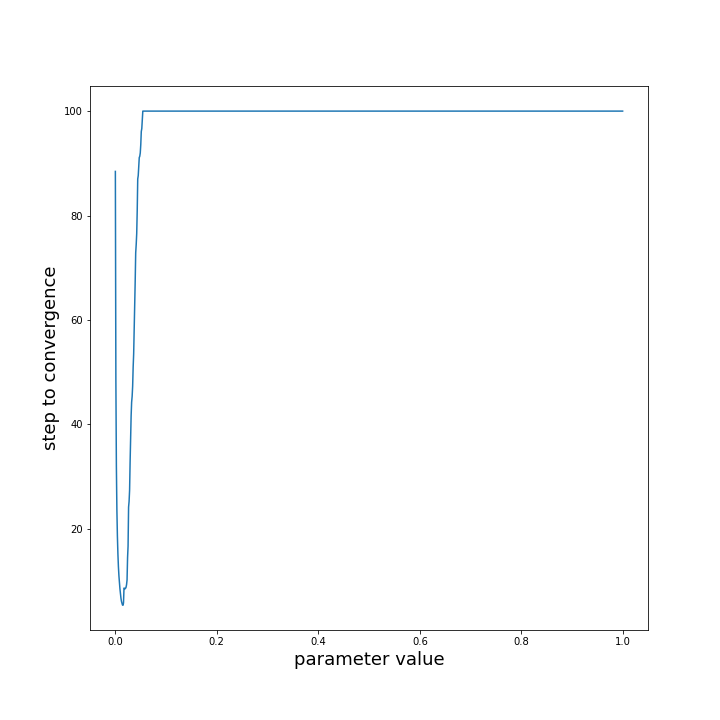
\includegraphics[width=1\textwidth]{fixed_step_parameter_poincare.png}
    \caption{Sequenza relativa alla convergenza del'algoritmo a passo fisso implementato su disco. Punto di minimo $0.27$, valore di convergeza minimo $7.35$.}
\end{figure}
\begin{figure}[H] %inserisce le figure
    \centering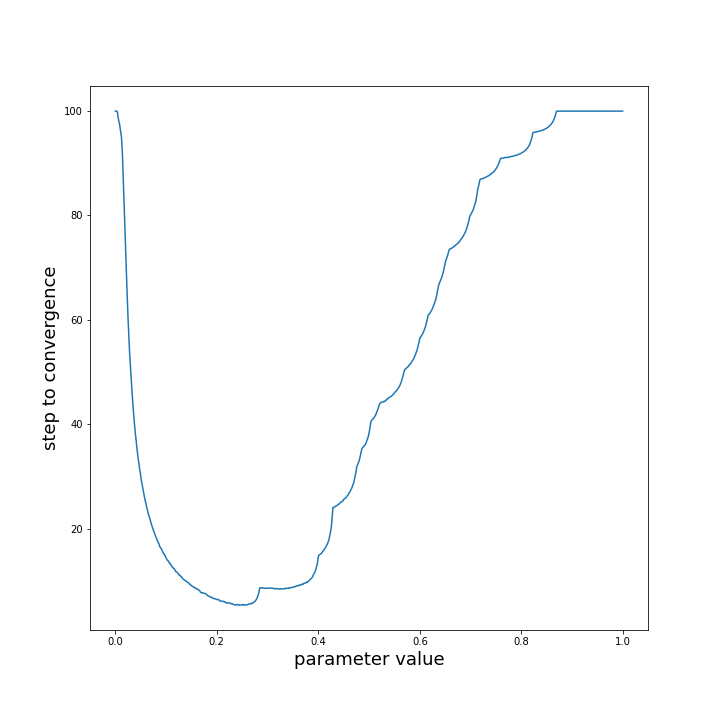
\includegraphics[width=1\textwidth]{fixed_step_parameter_hyperboloid.png}
    \caption{Sequenza relativa alla convergenza del'algoritmo a passo fisso implementato su iperboloide. Punto di minimo $0.27$, valore di convergeza minimo $7.35$.}
\end{figure}
Analogamente, per quanto riguarda le sequenze definite dalla scelta di $\lambda$ per l'algoritmo di Armijo, si è notato un'andamento molto simile nelle due sequenze, anche in questo caso il punto di minimo coincide.\\
\begin{figure}[H] %inserisce le figure
    \centering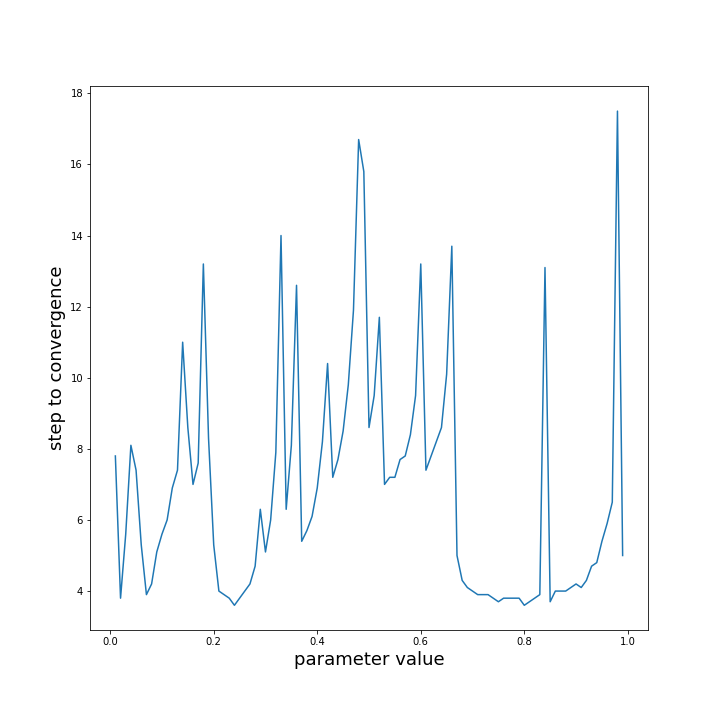
\includegraphics[width=1\textwidth]{armijo_parameter_poincare.png}
    \caption{Sequenza relativa alla convergenza del'algoritmo di Armijo implementato su disco. Punto di minimo $0.26$ , valore di convergeza minimo $7.9$.}
\end{figure}
\begin{figure}[H] %inserisce le figure
    \centering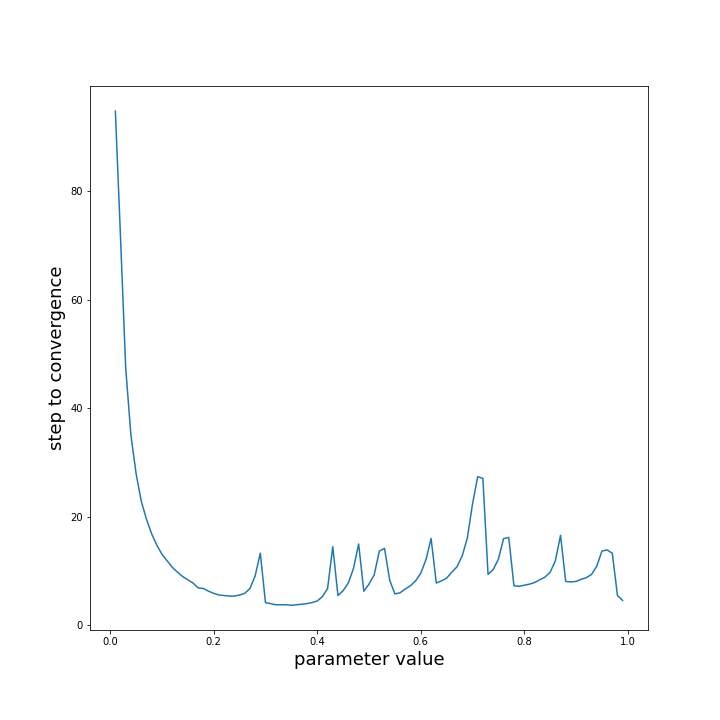
\includegraphics[width=1\textwidth]{armijo_parameter_hyperboloid.png}
    \caption{Sequenza relativa alla convergenza del'algoritmo di Armijo implementato su iperboloide. Punto di minimo $0.26$ , valore di convergeza minimo $7.9$.}
\end{figure}
A questo punto, avendo scelto i parametri che permettono ai nostri algoritmi di performare al meglio, possiamo procedere con il confronto.\\
Riprendendo il dataset totale, per ogni algoritmo lo abbiamo eseguito su ogni istanza del dataset, sia per l'implementazione su disco che per quella su iperboloide, creando un punto  ($a$, $b$) in $R^2$, per ogni istanza, le cui coordinate sono $a$, il numero di passi per convergere al punto limite per l'implementazione su disco, $b$ invece, il numero di passi per convergere al punto limite per l'implementazione su iperboloide, creando cosi una nuvola di punti.\\
Tramite tale nuvola possiamo verificare se le metodologie sono effettivamente equivalenti, in ogni grafico vengono inoltre costruite due rette di regressione su una versione ridotta della nuvola di punti, toglieremo quei punti che hanno una molteplicità bassa (e.g. sotto $\frac{1}{40}$ della cardinalità totale del dataset), la prima retta di regressione viene calcolata tramite il metodo dei minimi quadrati, la seconda invece viene calcolata tramite un algoritmo meno sensibile ai valori anomali, la regressione di $Huber$. Noteremo quindi che, se le rette di regressione tendono ad avere un coefficiente angolare "vicino" ad $1$ le due varietà possono essere ritenute equivalenti.  Riportiamo di seguito i grafici dei nostri esperimenti, verrà riportato, per ogni grafico, un valore medio di convergenza per il disco e per l'iperboloide, tale valore rappresenterà un ulteriore indice di confronto.\\
\begin{figure}[H] %inserisce le figure
    \centering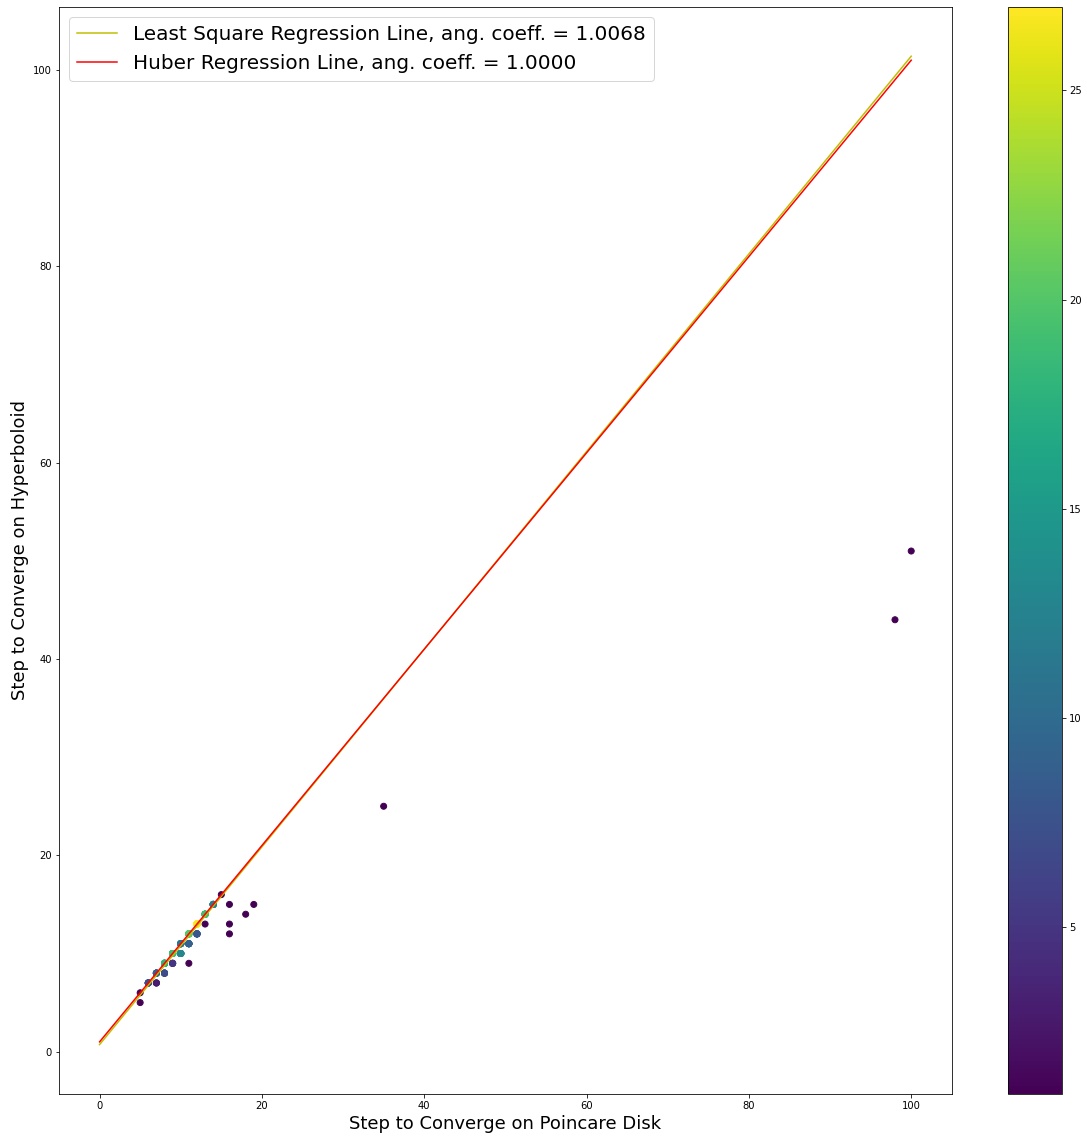
\includegraphics[width=1\textwidth]{fixed_step_size.png}
    \caption{Nuvola di punti relativa all'algoritmo a passo fisso, notiamo che i punti generati tendono a giacere sulla bisettrice, ciò indica un'equvalenza tra le due implementazioni. Valore medio di convergenza sul disco $10.5$, valore medio di convergenza su iperboloide $11.2$.}
\end{figure}
\begin{figure}[H] %inserisce le figure
    \centering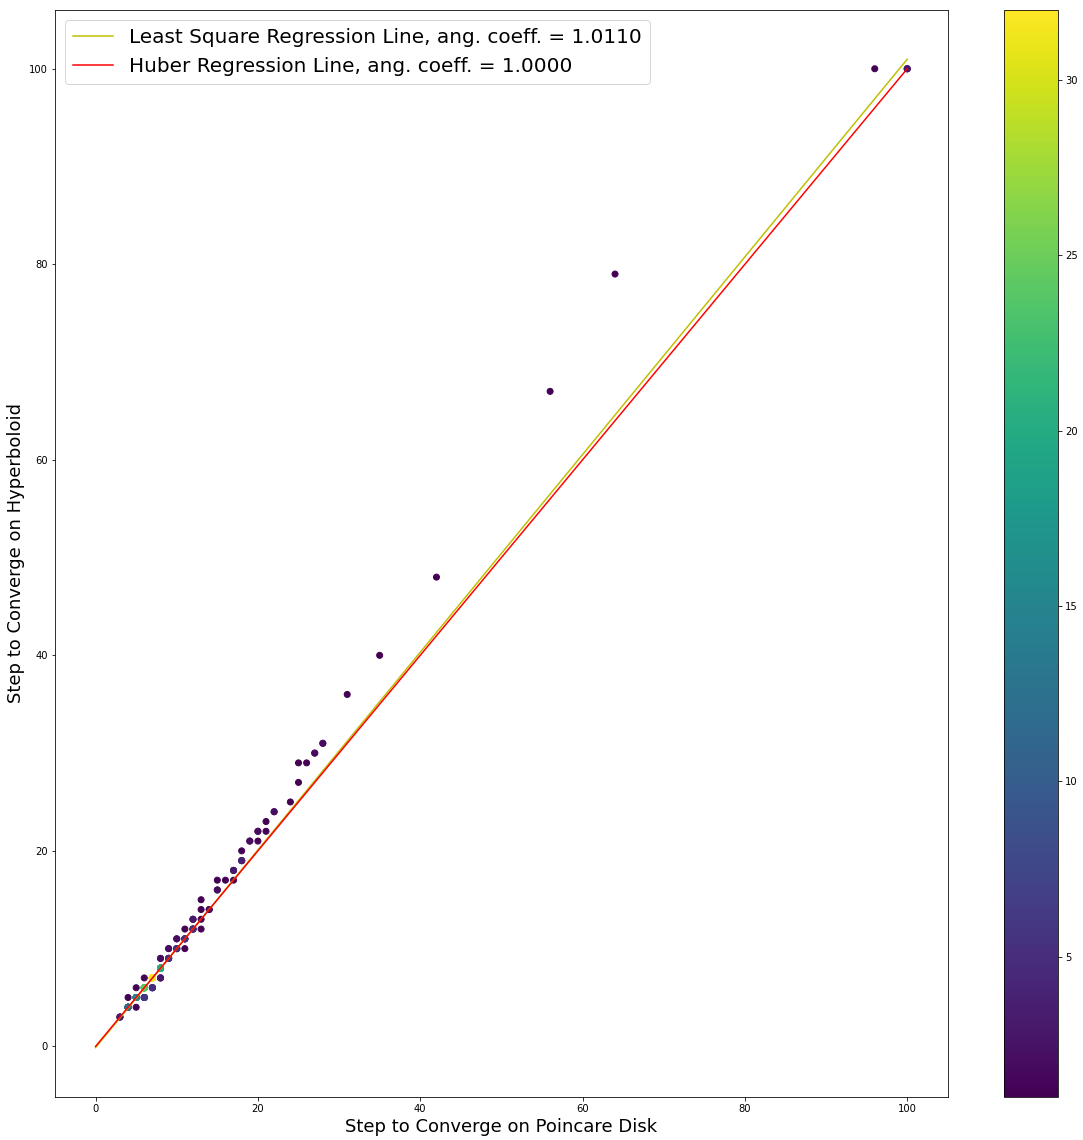
\includegraphics[width=1\textwidth]{armijo.png}
    \caption{Nuvola di punti relativa all'algoritmo di Armijo, notiamo che i punti generati tendono a giacere sulla bisettrice, ciò indica un equvalenza tra le due implementazioni. Valore medio di convergenza sul disco $10.4$, valore medio di convergenza su iperboloide $11.2$.}
\end{figure}
\begin{figure}[H] %inserisce le figure
    \centering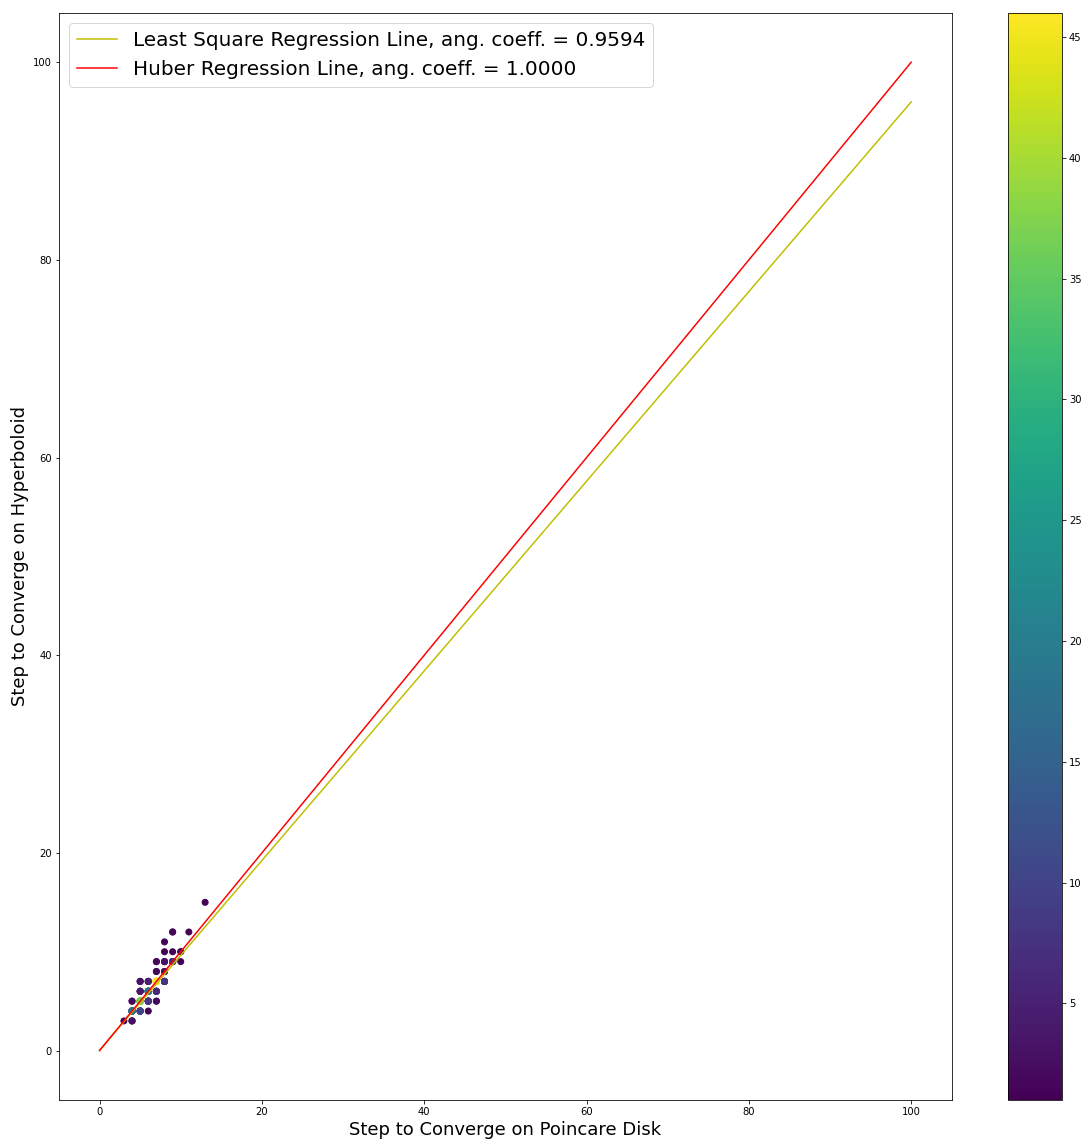
\includegraphics[width=1\textwidth]{barzilai_borwein.png}
    \caption{Nuvola di punti relativa all'algoritmo di Barzilai-Borwein, notiamo che i punti generati tendono a giacere sulla bisettrice, ciò indica un equvalenza tra le due implementazioni. Valore medio di convergenza sul disco $6.13$, valore medio di convergenza su iperboloide $6.8$.}
\end{figure}
Durante le nostre sperimentazioni ci siamo resi conto che il grafico relativo all' algoritmo di Barzilai-Borwein tende ad avere i coefficienti delle rette di regressione "molto vicini" ad $1$, ma non tutti i punti della nuvola tendono a giacere sulla bisettrice. Mentre i grafici relativi all'algoritmo di Armijo e l'algoritmo a passo fisso presentano una retta di regressione quasi equivalente alla bisettrice, e graficamente è facile vedere come tutti i punti, a meno di casi anomali, giacciono sulla bisettrice. Relativamente ai valori medi di convergenza, abbiamo valori abbastanza simili per tutti e tre gli algoritmi, possiamo notare una differenza di al più un passo e mezzo di differenza nella convergenza media.\\
Possiamo asserire che le implementazioni su disco e su iperboloide, degli algoritmi ottimizzazzione per il calcolo della media di Fréchet, sono pressoché equivalenti, i risultati di tali sperimentazioni ci portano a congetturare che, dato un problema di ottimizzazione su una varietà è possibile trasferire il problema da tale varietà ad una varietà conforme, tenendo presente che deve essere preservata l'esistenza di una soluzione ottima per la funzione da ottimizzare.\\
Concludendo, come è stato riportato nell'introduzione, un altro risultato delle nostre sperimentazioni è stato far vedere come l'algoritmo di Barzilai-Borwain si comporta meglio rispetto agli algoritmi di ricerca lineare, facendo riferimento al valore di convergenza medio, delle implementazioni sulle due varietà, riportate nelle descrizioni dei grafici.
Riportiamo il link alla repository Github contenente i codici degli esperimenti: \textit{https://github.com/Andrew-Wyn/Tesi\_Ottimizzazione}.
\section{Appendice}
Richiamiamo qui alcuni concetti teorici necessari per la piena comprensione del presente elaborato.
\subsection{Varietà}
Sia $M$ un insieme. Una bigezione $\psi$ differenziabile di un sottoinsime $U$ di $M$ in un sottoinsieme aperto di $\mathbb{R}^d$ è chiamata mappa $d$-dimensionale dell'insieme $U$ che definisce una \textit{carta} $(U, \psi)$. Data una carta $(U, \psi)$ e $x \in U$ gli elementi di $\psi(x) \in \mathbb{R}^d$ sono le coordinate di $x$ nella carta $(U, \psi)$. Un \textit{Atlante} $(A)$ di $M$ in $R^d$ è un insieme di carte $(U_a, \psi_a)$ dell'insieme $M$, dove $a$ varia in un insieme di indici $\mathcal{A}$, tali che:
\begin{itemize}
    \item $\bigcup_a U_a = M$, per $a \in \mathcal{A}$.
    \item Per ogni coppia $\alpha, \beta \in \mathcal{A}$ con $U_{\alpha} \cap U_{\beta} \neq \emptyset$ gli insiemi $\psi_{\alpha}(U_{\alpha} \cap U_{\beta})$ e $\psi_{\beta}(U_{\alpha} \cap U_{\beta})$ sono sottoinsiemi aperti di $R^d$ ed il cambio di coordinate $\psi_{\alpha} \circ \psi_{\beta}^{-1}:$ $\mathbb{R}^d \to \mathbb{R}^d$ è differenziabile.
\end{itemize}
Dato un'atlante $A$, sia $A^+$ l'insieme delle carte $(U, \psi)$ tali che $A \bigcup \{(U, \psi)\}$ è ancora un'atlante. $A^+$ è un'atlante massimale generato da $A$. Un'atlante massimale dell'insieme $M$ è chiamato struttura differenziabile su $M$.
\begin{definition}
Una varietà differenziabile $d$-dimensionale è una coppia $(M, A^+)$, dove $M$ è un insieme e $A^+$ è un atlante massimale su $M$ in $R^d$, tale che la topologia indotta da $A^+$ è di Hausdorff.
\end{definition}
Data una carta $\psi$ su $M$, l'inversa $\psi^{-1}$ è chiamata parametrizzazione locale di $M$.
\subsubsection{Vettori Tangenti}
Riprendendo il concetto di derivata direzionale possiamo generalizzarla per un funzione $f$ definita su una varietà, sustituendo $t \mapsto (x + t\eta)$ con una curva, $\gamma: U \to M$, con $0 \in U$ ed $\gamma (0) = x$, attraverso $x \in M$ (punto di derivazione) questo porta ad una derivata direzionale ben definita $\frac{\partial f(\gamma (t))}{\partial t} \vert_{t=0}$. Formalmente, sia $M$ una varietà e $\gamma$ una mappa differenziabile $\gamma : U \to M | t \mapsto \gamma (t)$ detta curva in $M$, data, una funzione $f$ a valori reali definita su $M$, la funzione $f \circ \gamma : t \mapsto f(\gamma (t))$ è una funzione differenziabile da $\mathbb{R}$ in $\mathbb{R}$ con una ben definita derivata.\\
Sia $x \in M$; $\gamma (0) = x$ allora indichiamo con $\mathcal{F}_{x}(M)$ l'insieme delle funzioni reali differenziabili definite in un intorno di $x$. Il mapping $\dot{\gamma} (0)$ da $\mathcal{F}_x(M)$ in $R$ è definito come: $\dot{\gamma} (0) f = \frac{\partial f(\gamma (t))}{\partial t} \vert_{t=0}$ con $f \in F_x(M)$; é chiamato vettore tangente alla curva $\gamma$ in $t=0$.
\begin{definition}[Vettore Tangente]
Un vettore tangente $\varepsilon_x$ ad una varietà $M$ in un punto $x \in M$ è una mappa da $F_x(M)$ in $R$ tale che esiste una curva $\gamma$ a valori in $M$ con $\gamma (0) = x$ e che soddisfa,\\
\[\varepsilon_xf = \dot{\gamma (0)} f = \frac{\partial f(\gamma (t))}{\partial t} \vert_{t=0} \quad  f \in F_x(M).\]\\
\end{definition}
Tale curva $\gamma$ realizza il vettore tangente $\varepsilon_x$.
\begin{definition}[Spazio Tangente]
Lo spazio tangente ad $M$ in $x$ denominato come $T_xM$ è l'insieme di tutti i vettori tangenti ad $M$ in $x$. Questo insieme ammette una struttura di spazio vettoriale come segue: date $\dot{\gamma}_1 (0)$ e $\dot{\gamma}_2 (0)$ in $T_xM$ e $a, b$ in $R$ allora,\\
\[(a \dot{\gamma}_1 (0) + b \dot{\gamma}_2 (0)) f = a (\dot{\gamma}_1 (0) f) + b (\dot{\gamma}_2 (0) f).\]
\end{definition}
Lo spazio tangente $T_xM$ mette a disposizione un'approssimazione locale della varietà tramite uno spazio vettoriale. Perciò tramite le retrazioni definite nella sezione \ref{retraction} possiamo effettuare ottimizzazione sullo spazio vettoriale $T_xM$.
\begin{definition}[Fibrato tangente]
Data una varietà $M$, sia $TM$ l'insieme di tutti i vettori tangenti ad $M$.\\
\[TM = \bigcup_{x \in M} T_xM.\]
\end{definition}
Sia $P:M \to N$ una mappa differenziabile tra due varietà $M$ ed $N$. sia $\varepsilon_x$ un vettore tangente in un punto $x$ di $M$, si può far vedere che $DP(x)[\varepsilon_x]$ da $F_{P(x)}(N)$ in $\mathbb{R}$ è definita da:\\
\[(DP(x)[\varepsilon_x])f = \varepsilon_x(f \circ P),\]\\
è un vettore tangente ad $N$ in $P(x)$.\\
La mappa $DP(X) : T_xM \to T_{P(x)}N | \varepsilon_x \mapsto DP(x)[\epsilon_x]$ è una mappa lineare chiamata differenziale di $P$ in $x$.
\subsubsection{Metriche distanze e gradienti riemanniani}
I vettori tangenti ad una varietà generalizzano la nozione di derivata direzionale. Questo può essere fatto munendo lo spazio tangente $T_xM$ con un prodotto interno $\langle \cdot, \cdot \rangle_x$ bilineare, definito positivo e simmetrico. Il prodotto interno induce una norma $\| \varepsilon_x \|_x = \sqrt{\langle \epsilon_x, \epsilon_x \rangle_x}$ su $T_xM$. Una varietà il cui spazio tangente è munito di un prodotto interno, che dipende in modo differenziabile da $x$, prende il nome di varietà riemanniana $(M, g)$ con $g$ metrica riemanniana.\\
La lunghezza di una curva $\gamma:[a,b] \to M$ in una varietà riemanniana $(M, g)$ è definita da,\\
\[L(\gamma) = \int_a^b \sqrt{g(\dot{\gamma} (t), g(\dot{\gamma} (t)))}.\]\\
La distanza riemanniana in una varietà riemanniana connessa $(M,g)$ è $\mathrm{dist}: M \times M \to \mathbb{R} \, | \, \mathrm{dist}(x,y) \mapsto \inf_{\gamma \in \Gamma}(L(\gamma))$, dove $\Gamma$ è l'insieme di tutte le curve in $M$ che connettono $x$ ed $y$.\\
Sia $f$ la solita funzione liscia definita su $(M,g)$, il gradiente riemanniano di $f$ in $x$ è definito come l'elemento di $T_xM$ che soddisfa,\\
\[\langle \nabla^{(R)} f(x), \epsilon \rangle_x = Df(x)[\epsilon].\]\\
Sia $M$ una sottovarietà immersa di una varietà riemanniana $\widehat{M}$ siccome ogni spazio tangente $T_xM$ può essere trattato come sottospazio di $T_x\widehat{M}$ la metrica $\widehat{g}$ di $\widehat{M}$ induce una metrica $g$ su $M$, $g_x(\xi, \eta) = \widehat{g}_x(\xi, \eta)$ con $\xi, \eta \in T_xM$, perciò $M$ è una sotto varietà riemanniana.
\subsection{Topologia}
Una topologia su un insieme $X$ è una collezione $T$ di sottoinsiemi di $X$ chiamati insiemi aperti, tali che:
\begin{itemize}
    \item $X$ e $\emptyset$ appartengono a $T$.
    \item L'unione di elementi di qualsiasi sotto collezione di $T$ è in $T$.
    \item L'intersezione di elementi di qualsiasi sotto collezione finita di $T$ è in $T$.
\end{itemize}
Uno spazio topologico è una coppia $(X,T)$ dove $X$ è un insieme e $T$ è una topologia su $X$.
\begin{definition}[Hausdorff]
Un insieme $X$ è $T_2$ o di Hausdorff se ogni coppia di punti distinti di $X$ ammettono intorni distinti.
\end{definition}
Se $X$ è di Hausdorff allora ogni sequenza di punti di $X$ converge ad al più un punto di $X$.
\subsection{Miscellanea}
\begin{definition}[Positività]
Sia $A \in \mathbb{R}^{n \times n}$ è definita positiva se è simmetrica e se $v'Av > 0$ se $v$ è un vettore $\in \mathbb{R}^n \setminus \{0\}$.
\end{definition}
Si osservi che se $v = 0$ allora che $v'Av = 0$.
\begin{definition}[Convessità]
Una funzione $f:\Omega \to \mathbb{R}$ con $\Omega \subset V$, $V$ (spazio vettoriale) ed $\Omega$ convesso, è definita convessa se: $(f((\lambda)v + (1 - \lambda)w) \leq \lambda f(v) + (1 - \lambda)f(w)$, per $\lambda \in [0;1]$ e $v, w \in \Omega$.
\end{definition}
\begin{definition}[Derivate Parziali]
Data una funzione $f:V \to \mathbb{R}$, $V$ (spazio vettoriale), allora una derivata parziale su $x \in V$ è definita come:\\
\[\frac{\partial f(x)}{\partial x_i} = \lim_{h \to 0} \frac{f(x + h e_i) - f(x)}{h};\]\\ 
con $x_i$ componente i-esima di $x$ ed $e_i$ i-esimo vettore della base canonica.\\
\end{definition}
Se una funzione è differenziabile in $x$ allora tutte le derivate parziali esistono in $x$.
\begin{definition}[Punto di accumulazione]
Diciamo che $x \in \mathbb{R}$ è un punto di accumulazione per un insieme $E \subset \mathbb{R}$ se comunque scelto un intorno $B(x, \epsilon)$, risulta che $B(x, \varepsilon)$ contiene almeno un punto di $E$ diverso da $x$.
\end{definition}
\begin{definition}[Gradiente]
Consideriamo una funzione $f$ definita su un insieme aperto $A \subset \mathbb{R}^n$ e sia $x \in A$ se esistono in $x$ le derivate parziali rispetto ad $\{x_i\}_{i=1, ..., n}$ allora è possibile costruire un vettore che ha per componenti le derivate parziali, perciò il gradiente è definito come.\\
\[\nabla f(x) = \left[\frac{\partial f(x)}{\partial x_1}, ..., \frac{\partial f(x)}{\partial x_n}\right].\]
\end{definition}
Inoltre per la formula del gradiente sappiamo che, dato un versore $v$ esiste la derivata direzionale $f_v$ in $x$ e che $f_v(x) = \nabla f(x) \cdot v$.
\newpage

\bibliographystyle{unsrt}
\bibliography{bibliografia}

\end{document}

\begin{thebibliography}{9}
\bibitem{Gradient Descent in Hyperbolic Space}
Benjamin Wilson and Matthias Leimeister.
\textit{Gradient Descent in Hyperbolic Space}.

\bibitem{Hyperbolic Entailment Cones for Learning Hierarchical Embeddings} 
Octavian-Eugen Ganea, Gary Becigneul and Thomas Hofmann.
\textit{Hyperbolic Entailment Cones for Learning Hierarchical Embeddings}.

\bibitem{Poincare for Learning Hierarchical Representations}
Maximilian Nikel and Douwe Kiela.
\textit{Poincaré for Learning Hierarchical Representations}.

\bibitem{Iannazzo} 
Bruno Iannazzo and Margherita Porcelli.
\textit{The Riemannian BARZILAI-BORWEIN METHOD WITH NONMONOTONE LINE SEARCH AND THE MATRIX GEOMETRIC MEAN COMPUTATION}.

\bibitem{GeoOpt} 
GeoOpt: Python Library for Manifold Optimization,
\\\texttt{https://geoopt.readthedocs.io/en/latest/}

\bibitem{ManOpt} 
Manopt: Python Library for Manifold Optimization,
\\\texttt{https://www.manopt.org/}

\end{thebibliography}